\let\negmedspace\undefined
\let\negthickspace\undefined
\documentclass[journal]{IEEEtran}
\usepackage[a5paper, margin=10mm, onecolumn]{geometry}
\usepackage{gvv-book}
\usepackage{gvv}
\usepackage{cite}
\usepackage{amsmath,amssymb,amsfonts,amsthm}
\usepackage{graphicx}
\usepackage{mathtools}
\usepackage{tkz-euclide}

\title{10.3.3}
\author{EE25BTECH11005 - Aditya Mishra}

\begin{document}

\maketitle

\textbf{Question}:\\
Find the equation of the normal lines to the curve 
\[
3x^2 - y^2 = 8
\] 
which are parallel to the line 
\[
x + 3y = 4.
\]

\textbf{Solution:}\\

The general equation of a conic is 
\begin{align}
\vec{x}^\top \vec{V} \vec{x} + 2\vec{u}^\top \vec{x} + f = 0
\end{align}

Comparing with $3x^2 - y^2 = 8$, we get
\begin{align}
\vec{V} = \myvec{3 & 0 \\ 0 & -1},\quad
\vec{u} = \myvec{0 \\ 0},\quad
f = -8
\end{align}

The slope of the line $x + 3y = 4$ is $-\frac{1}{3}$, so the normal vector of the required normals is
\begin{align}
\vec{n} = \myvec{1 \\ 3}
\end{align}

The points of contact of normals with a given normal vector are
\begin{align}
\vec{q}_i = \vec{V}^{-1} (k_i \vec{n} - \vec{u}), \quad i = 1,2
\end{align}
where $k_i$ satisfy
\begin{align}
k^2 \vec{n}^\top \vec{V}^{-1} \vec{n} - 2 k \vec{u}^\top \vec{V}^{-1} \vec{n} + \vec{u}^\top \vec{V}^{-1} \vec{u} + f = 0
\end{align}

Here,
\begin{align}
\vec{V}^{-1} = \myvec{\tfrac{1}{3} & 0 \\ 0 & -1}, \quad
\vec{n}^\top \vec{V}^{-1} \vec{n} = \myvec{1 & 3} \myvec{\tfrac{1}{3} & 0 \\ 0 & -1} \myvec{1 \\ 3} = -\frac{26}{3}
\end{align}

Substituting in the quadratic equation:
\begin{align}
k^2 \left(-\frac{26}{3}\right) - 8 = 0
\quad \Rightarrow \quad k = \pm 3\sqrt{3}
\end{align}

The points of contact are
\begin{align}
\vec{q}_i = \vec{V}^{-1} (k_i \vec{n})
= \myvec{\tfrac{k_i}{3} \\ -3 k_i}
\end{align}

Substituting $k_1 = 3\sqrt{3},\ k_2 = -3\sqrt{3}$, we get
\begin{align}
\vec{q}_1 = \myvec{\sqrt{3} \\ -9\sqrt{3}}, \quad
\vec{q}_2 = \myvec{-\sqrt{3} \\ 9\sqrt{3}}
\end{align}

The equation of the normal at $\vec{q}_i$ is
\begin{align}
\vec{n}^\top (\vec{x} - \vec{q}_i) = 0
\quad \Rightarrow \quad
\vec{n}^\top \vec{x} = \vec{n}^\top \vec{q}_i
\end{align}

Hence, the required normals are
\begin{align}
x + 3y &= \vec{n}^\top \vec{q}_1 = -26\sqrt{3} \\
x + 3y &= \vec{n}^\top \vec{q}_2 = 26\sqrt{3}
\end{align}

\[
\boxed{x + 3y = \pm 26\sqrt{3}}
\]
See Figure,
\begin{figure}[h!]
    \centering
    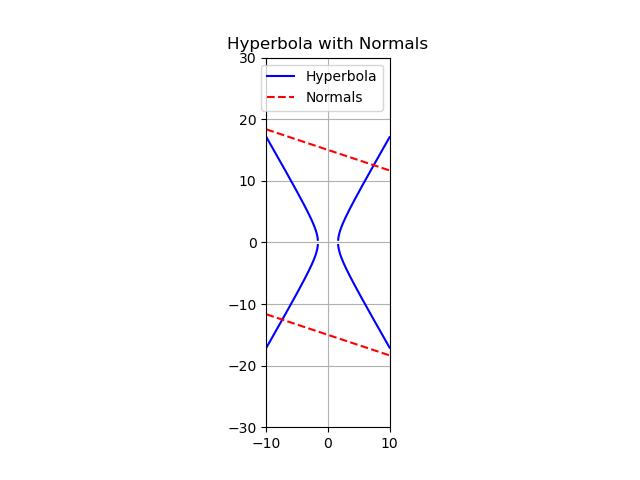
\includegraphics[height=0.5\columnwidth, keepaspectratio]{Figs/Figure_1.png}
    \label{figure_1}
\end{figure}
\end{document}

